\chapterimage{glass_ball}
\chapter{Prediction}\label{sec:prediction}

The goal of this chapter is to illustrate the utility of a prediction stage
in data compression pipelines, and some of the main realizations.

\section{Residuals}

Except for a brief digression in Chapter~\ref{sec:coding:adaptativity}, symbols produced by a source \source have been assumed to be \conceptRef{independence}{independent}. However, this does not hold for most real sources. For instance, the next word in a sentence is strongly biased by the previous characters, and image pixels tend to be similar to their neighbors and across \conceptRef{band}{bands}.
We can then say that there is \concept{redundancy} present among those samples.

A \concept{prediction} stage can be inserted before entropy coding to remove some of that redundancy with the hope that \concept{entropy} is reduced. For each input sample $x$, the prediction stage ``bets'' on its most likely value $\hat{x}$ looking only at previously transmitted data (\ie, using a \concept{causal context}). Then, the \concept{prediction residual} $\Delta = x - \hat{x}$ is computed, encoded and transmitted.
%
The receiver should be able to reproduce the same predicted values $\hat{x}$ and combine them with the transmitted residuals to reconstruct the original value as $x = \Delta + \hat{x}$.

The \conceptRef{causal context}{context} used for prediction can be as small or as large as the computational and memory constraints permit. These contexts can be 1D, 2D, 3D, 4D and beyond depending on the dimensionality of the input data (see for instance an example video prediction scheme below). They can also use a priori information about the dataset (\eg, the average sample value). Whatever the context, the \conceptRef{causal context}{causality} constraint is critical for the receiver to be able to reproduce the same predicted values $\hat{x}$.

\begin{center}
    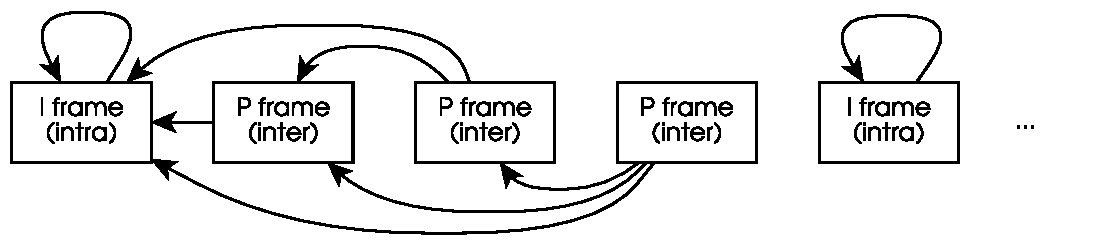
\includegraphics[width=0.8\linewidth]{video_prediction_scheme}
\end{center}

\begin{wrapfigure}{L}{5cm}
\begin{tikzpicture}
\begin{axis}[
    axis lines=middle,
    axis line style={-},
    xtick=\empty,
    ytick=\empty,
    xlabel={},
    ylabel={},
    domain=-5:5,
    samples=200,
    width=6cm,
    height=8cm,
    enlargelimits=true,
    clip=true,
    color=color2,
]
\addplot[color1, thick] {0.5 * exp(-abs(x)/0.25)};
\end{axis}
\end{tikzpicture}

\end{wrapfigure}

A good predictor, assuming samples are highly \conceptRef{correlation}{correlated} (high \concept{redundancy}), produces many zero-valued residuals. The probability of $\pm 1$ residuals, $\pm 2$ residuals, etc., decays quickly, yielding a distribution akin to a \mbox{\conceptRef{Laplacian distribution}{Laplacian}}.\\
%
The better the predictor, the sharper the distribution shape and the lower the entropy of the resulting residuals.

Getting acquainted with this distribution is very useful in the context of data compression because of its high prevalence: it is not only produced by good predictions, but is also a good description of the coefficients produced by the \conceptRef{discrete cosine transform (DCT)}{discrete cosine transforms (DCT)} and \conceptRef{discrete wavelet transform (DWT)}{discrete wavelet transforms (DWT)} explored in Chapter~\ref{sec:transforms}.

Information about this distribution is critical to design well-performing entropy coders, adaptive or not, as discussed in Chapter~\ref{sec:coding}. It also motivates the use of \concept{deadzone quantization}, as introduced in Chapter~\ref{sec:quantization:examples}.

\section{Linear and nonlinear}

Prediction functions are often \concept{linear} because of their implementation and optimization properties. Notwithstanding, they can also be non-linear as long as they can be perfectly replicated by the decoder.

The causal context can be employed to choose one among several possible predictors. The PPM~\cite{cleary_ppm} and LZ~\cite{lz77} (see Chapter~\ref{sec:coding:adaptativity}) families of compressors exploit this fact, attempting to find perfect matches of variable length. These are chiefly useful for the compression of text data and other sources with small alphabets, especially when produced by a \concept{grammar}. In turn, the PAQ~\cite{mahoney_paq1} family of compressors tries multiple approaches and combines them using \concept{context mixing}.

\begin{remark}
Some of the algorithms in the previous paragraph are used to drive the probabilities of an adaptive arithmetic coder, but are included in this section by affinity.
\end{remark}

Another popular, nonlinear approach to prediction is to define piece-wise functions. Depending on which of a number of mutually-exclusive conditions is met by the causal context, a different prediction expression is used. This condition can, for instance, attempt to identify ``flat'' versus ``edge'' regions, and predict accordingly. Two main examples of this approach are CALIC~\cite{wu_calic} and JPEG-LS~\cite{jpeg_ls}. The prediction function of the latter can be expressed as follows:

\begin{minipage}{0.2\linewidth}
\begin{center}
\begin{tabular}{c|c|c}
C & B & D \\
\midrule
A & $\hat{x}$\\
\end{tabular}
\end{center}
\end{minipage}%
\begin{minipage}{0.7\linewidth}
$$
\hat{x} = \left\{
\begin{array}{lp{0.5cm}l}
\min(A,B) & & \textrm{if}\ C \ge \max(A,B) \\
\max(A,B) & & \textrm{if}\ C \le \min(A,B) \\
A + B - C & & \textrm{otherwise}
\end{array}
\right..
$$
\end{minipage}

Regardless of the prediction method employed (assuming those predictions are reasonable), it is possible to map each residual $\Delta$ into the original data's \concept{dynamic range}, $\Delta \mapsto \delta$. Equations (55) and (56) of~\cite[\S 4.11]{ccsds123x0b2} describe one such way -- a slightly simplified version for positive integers is shown next following the previously employed notation.
Note how this mapping function requires not only the prediction residual, but also the value of the prediction itself.
%
\begin{eqnarray*}
\theta(\hat{x}) &=& \min(\hat{x} - x_\textrm{min}, x_\textrm{max} - \hat{x}) \\
\Delta(x, \hat{x}) &=& x - \hat{x} \\
\delta(x, \hat{x}) &=& \left\{
\begin{array}{ll}
\theta + |\Delta|  & \textrm{if}\ \hat{x} > \theta \\
2|\Delta| &  \textrm{if}\ |\Delta| \le \theta\ \textrm{and}\ |\Delta|\ \textrm{is even} \\
2|\Delta| -1  & \textrm{if}\ |\Delta| \le \theta\ \textrm{and}\ |\Delta|\ \textrm{is odd} \\
\end{array}
\right.
\end{eqnarray*}

\begin{center}
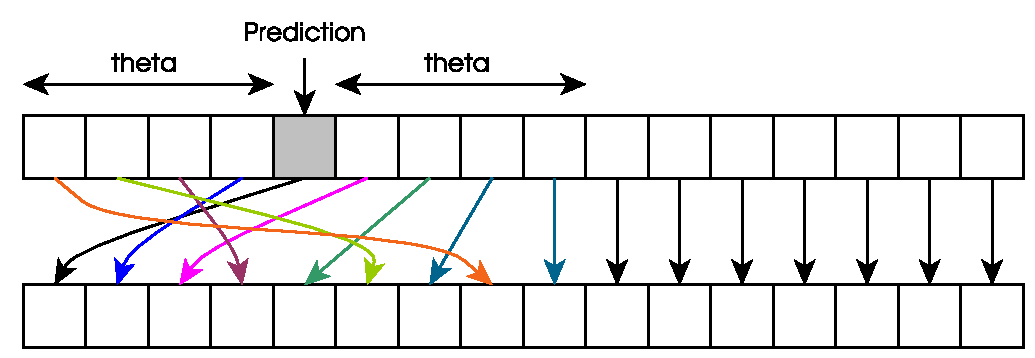
\includegraphics[width=0.75\linewidth]{residual_mapping}
\end{center}

A correctly applied prediction scheme does not introduce any data loss. That said, prediction can also be part of \concept{lossy compression} pipelines that involve a \concept{quantization} function $Q$. Quantization can be applied before or after prediction, introducing the same range of errors in both cases. Doing it before is computationally simpler, but rate-distortion theory predicts a lower \concept{mean squared error} if quantization is applied afterwards~\cite[\S 3.3]{taubman2002jpeg2000}.
%
Specifically, $\textrm{MSE}_\textrm{after} = ({\sigma_\textrm{residuals}^2}/{\sigma_\textrm{data}^2}) \textrm{MSE}_\textrm{before}$, where $\sigma_\textrm{residuals}^2$ and $\sigma_\textrm{data}^2$ are the variances of the original data and the prediction residuals, respectively.
%

The main drawback of applying quantization after prediction is the fact that the encoder needs to
replicate the dequantization process in the compression loop, and use the reconstructed sample values for prediction instead of the original. Otherwise, the encoder and the decoder would be using a different set of values as inputs to the prediction function, and the transmitted residuals (either $\Delta$ or $\delta$) would not guarantee proper reconstruction. The modified encoder-decoder loop is described in~\cite[\S 3.3]{taubman2002jpeg2000} and~\cite[\S 11.3]{sayood_introduction} and illustrated next:

\begin{center}
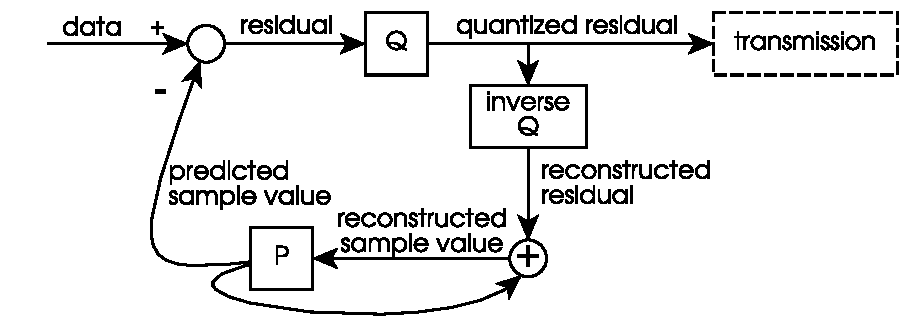
\includegraphics[width=0.75\linewidth]{prediction_quantization}
\end{center}


% \todo[inline]{TODO:}
% \begin{itemize}
% \item adaptive prediction ccsds 123, $R^-1$ (test it out actually)
% \item prediction + quantization vs quantization + prediction
% \item Organize exercises all sections: first theoretical, then practical
% \item fix the prediction and ml sections a bit?
% \end{itemize}



\section*{Further reading and practice}

\begin{itemize}
\item Cleary and Witten's paper~\cite{cleary_ppm} introduced one of the most successful and widely extended prediction approaches. A gentler description is also available in~\cite[\S 9.2]{mcanlis_understanding}.

\vspace{0.1cm}
\item The PAQ series, created by Mahoney, of algorithms use context mixing to provide slow but powerful prediction models. The original PAQ1 is introduced in~\cite{mahoney_paq1}, and further versions are referenced in the author's webpage~\url{https://mattmahoney.net/dc/}.
A good introduction to this family of algorithms is available in Salomon and Motta's book~\cite[\S 5.15]{salomon_handbook}.

\vspace{0.1cm}
\item The CCSDS~123.0-B-2 standard~\cite{ccsds123x0b2} contains a highly efficient (albeit somewhat complex) predictor that adapts
its weights based on the previously observed samples (and therefore the produced residuals).

\vspace{0.1cm}
\item Sayood's book~\cite[\S 8.6.2]{sayood_introduction} explains how to choose optimal linear prediction weights (in the MSE sense) based on the signal's autocorrelation.
\end{itemize}


\begin{exercise}
What's the highest and lowest entropy possible for a
scalar prediction scheme applied to a source \source?
\end{exercise}

\begin{exercise}
Using the notation $I_{x,y,z}$ to refer to a pixel in a color image,
provide the mathematical expression for a 1D, a 2D and a 3D predictor $\hat{I}_{x,y,z}$.
\end{exercise}

\begin{exercise}
In addition to natural text, what sources do you think could benefit from compression with LZ and/or PPM algorithms?
\end{exercise}

\begin{exercise}
How does the CALIC predictor compare to the LOCO-I used in JPEG-LS?
\end{exercise}

\begin{exercise}
Grab the mandrill image sample (\url{mandrill-u8be-3x512x512.raw})
and perform a simple, causal prediction.
\begin{itemize}
    \item What is the dynamic range of the residuals?
    \item What is the entropy of the resulting residuals?
    \item What parameters ($\mu$ and $b$) best model the resulting distribution?
    You may want to use the \texttt{curve\_fit} function described at \url{https://docs.scipy.org/doc/scipy/reference/generated/scipy.optimize.curve_fit.html}.
\end{itemize}
\end{exercise}

\begin{exercise}
Consider a sequence of data that begins with $137,\,39081,\,4829,\,\ldots$. Apply the $\hat{x}_i = x_{i-1}$ prediction function followed by a uniform scalar quantizer with $qstep=3$. Compare the obtained reconstruction errors for:
\begin{itemize}
\item the correct case that replicates the reconstruction process in the encoder, and
\item the incorrect case that doesn't.
\end{itemize}

\end{exercise}



